\section{Nova verzija programa}
U drugoj verziji poboljšana je vremenska kompleksnost tako što je uklonjena rekurzija te dodana
memoizacija. Nova vremenska kompleksnost je $O(N)$, dok je memorijska kompleksnost $O(1)$. Nova
verzija prikazana je kodom~\ref{04fibv2}. Također, u novoj verziji izmjenjen je dizajn, kao što je
prikazano slikom~\ref{fig:04redesign}

\lstset{caption={Fibonacci v2}, label=04fibv2}
\begin{lstlisting}[float=h]
func fibonacci(n uint64) uint64 {
	if n == 0 {
		return 0
	}
	a := uint64(0)
	b := uint64(1)

	for n > 1 {
		tmp := a + b
		a = b
		b = tmp
		n--
	}
	return b
}
\end{lstlisting}

\begin{figure}[h]
    \centering
    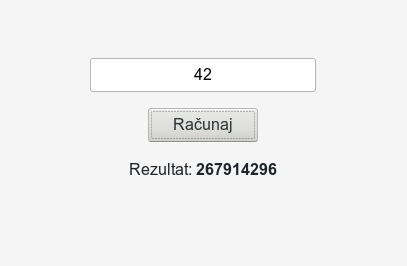
\includegraphics[width=0.5\textwidth]{img/04/new_app.png}
    \caption{Novi dizajn fibonacci aplikacije}%
    \label{fig:04redesign}
\end{figure}

Čim se takva izmjena spremljena na Github unutar glavne, \textit{master} grane, Jenkins pokreće
izgradnju nove aplikacije. Ukoliko su svi testovi budu uspješni, Docker slika se objavljuje. Zatim
servis za menadžment dohvaća novu verziju te počinje posluživati korisnike s novom verzijom.

Prethodnu verziju aplikacije potrebno je ukloniti tek nakon što su svi zahtjevi obrađeni. Na
primjer, ukoliko je potrebno 2 sekunde za obradu nekog zahtjeva tada je potrebno pričekati barem
toliko vremena prije nego što se prethodna verzija aplikacije može potpuno ugasiti. Uprotivnom,
zahtjev korisnika neće biti potpuno ispunjen.

Testiranje stabilnosti aplikacije prilikom izmjene koda provedeno je alatom \textit{Jmeter}. Jmeter
je alat za stresno testiranje aplikacije, a razvija ga neprofitna organizacija \textit{Apache}. Može
se koristiti za stresno testiranje baza podataka preko JDBC, FTP, LDAP, HTTP, i mnogih drugih
protokola.

Za testiranje infrastrukture ovog projekta korišten je HTTP protokol. Izvršeno je 10.000 zahtjeva
za 34.~fibonaccijev broj. U trenutku pokretanja stresnog testa, korištena je stara verzija fibonacci
aplikacije. Zatim je objavljena nova verzija sa optimizacijom. Svi zahtjevi uspješno su izvršeni. Na
slici~\ref{fig:04stresstest} prikazan je vremenski odaziv prve i druge verzije aplikacije.

\begin{figure}[h]
    \centering
    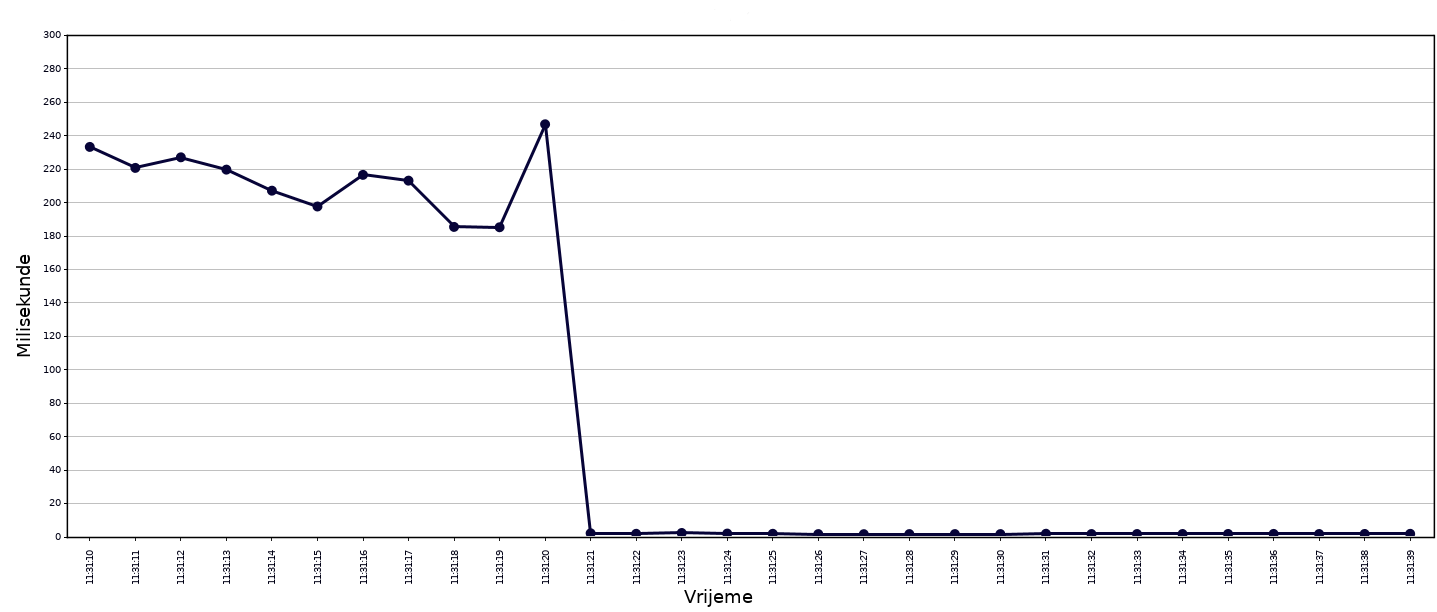
\includegraphics[width=\textwidth]{img/04/response_time.png}
    \caption{Vrijeme odaziva aplikacije}%
    \label{fig:04stresstest}
\end{figure}

\section{Vraćanje na staru aplikaciju}
Bilo koja izmjena aplikacije može uzrokovati neočekivanom greškom. Stoga, svaka izmjena aplikacije
predstavlja rizik. Korištenjem testova jedinica i \textit{end-to-end} testova povećana je
vjerojatnost otkrivanja greške prilikom razvoja aplikacije. Ukoliko novoobjavljena verzija
aplikacije sadrži neku grešku, potreban je dobar sustav da se takva greška može brzo otkloniti.
Često je najbrže rješenje vraćanje na staru verziju aplikacije (\textit{engl. version rollback}),
gdje se neispravna verzija zamjenjuje s prethodno objavljenom, stabilnom verzijom. Zatim je potrebno
ukloniti grešku u kodu te dodati prikladne testove nakon čega se može objaviti nova, ispravljena
verzija aplikacije.

U ovom radu korišten je parametrizitrani Jenkins posao za vraćanje na prethodno objavljenu verziju.
Prilikom pokretanja takvog posla, korisniku je dan padajući izbornik sa svim verzijama aplikacije.
Nakon što korisnik izabere željenu verziju, Jenkins označava tu verziju aplikacije kao zadnju.
Unutar trideset sekundi, servis za menadžment pokreće novoizabranu verziju aplikacije i počinje ju
posluživati. U tom trenutku, verzija aplikacije s greškom se ne poslužuje korisnicima.


